\documentclass[../main/main.tex]{subfiles}

\begin{document}

\section{Overview of exercises (PART I)}

\begin{enumerate}
\item limb-darkening scattering exercise we did during the course. 
— You can look into your notes from that, and I attach here also a sample program which you can use a base. After you have familiarised yourself with this, you can start to think bout how you would go about to extend this to a 3D setting (assuming isotropic scattering). 

\item (As prep for Monte-Carlo school) here is a script computing a UV resonance P-Cygni line in spherically symmetric wind with v beta-law. At top of routine, a few exercises are given, where you can modify and play around with code. Monte-Carlo program which computes a UV resonance spectral line from a fast outflowing spherically symmetric stellar wind (if you were not cc’d on that email, let me know so that I can send you the files as well). At the top of that little script, there are a few suggestions for exercises (additions) you could do to that program, in order to learn a bit more about the general workings of Monte-Carlo radiative transfer in this context.  
— So that might be a good idea for you to do as well !   (And you can also ask the others in the group for some tips etc. then.) 

\item Some background reading: 
\begin{itemize}
\item Attached mc manual by Puls. 
\item Paper by Sundqvist+ 2010 (Appendix, I think). 
\end{itemize}
\end{enumerate}


\section{Overview of exercises (PART II)}
\label{Overview_Part_2}

\begin{enumerate}
\item Calculate the probability distribution to sample from in the case of Eddington limb darkening for the initial distribution (see \ref{Eddington limb darkening adaptation}).
\item Calculate analytical solution for simplified problem in \ref{PCYG FIRST adaptation} in the case that \texttt{mu = 1}.
\item Perform convergence analysis. See Section \ref{convergence_analysis}
\end{enumerate}


\newpage
\section{Limb darkening}

\label{limb_darkening_discussion}

\subsubsection{2D Case}
We again have $\mu = \cos(\theta)$. The solution of the radiative transfer equation in \underline{plane-parallel syummetry} with frequency-independent absorption and emission, is 
\begin{equation}
I(\mu) = I_1 (0.4 + 0.6\mu)
\end{equation}
In the Monte Carlo code, the photons are sorted according to the direction that they leave the atmosphere.

\paragraph{Goal}
Calculates the angular dependence of photon's emitted from a plane-parallel, grey atmosphere of radial optical depth \texttt{taumax}. The value of \texttt{tau} determines the position of the photon

\paragraph{Variables and Algorithm}
\begin{itemize}
\item \texttt{muarray} contains emergent photons
\item \texttt{na} number of channels
\item \texttt{dmu} = 1/\texttt{na} width of channels
\item \texttt{nphot} number of photons
\item \texttt{taumax} maximum optical depth
\end{itemize}

\begin{algorithm}
\caption{Limb darkening: compute quantitiy of photons}\label{limb_darkening}
\begin{algorithmic}
\State initialization \\
\quad radial optical depth $\tau$ \\
\quad direction $\mu$

\For{all photons} 

\State $\boxed{\tau = \tau_{max}}$
	\While{\texttt{tau} $\geq 0$} 
	
	\State compute scattering angle \texttt{mu}
	\If{tau $\geq$ taumax} $\boxed{mu = sqrt(x)}$ (initial distribution)
	\Else{ $\boxed{mu = 2*x = 1}$} (isotropic scattering)
	\EndIf
	
	\State tau\_i = -log(x2) 
	\State tau = tau - tau\_i*mu	
		
	\EndWhile
	\State \textbf{end while}

	\State now we know that the photon has left the photosphere	
	\State compute the distribution of all angles \texttt{mu} at which the photon left the photosphere
	
\EndFor
\State \textbf{end for}

\State visualisation: 
	\begin{itemize}
	\item plot photon numbers from $\mu d\mu$ against \texttt{mu}
	\item plot specific intensity from $d\mu$ against \texttt{mu} against 
	\end{itemize}


\end{algorithmic}
\end{algorithm}


\begin{figure}[!htp]
\centering
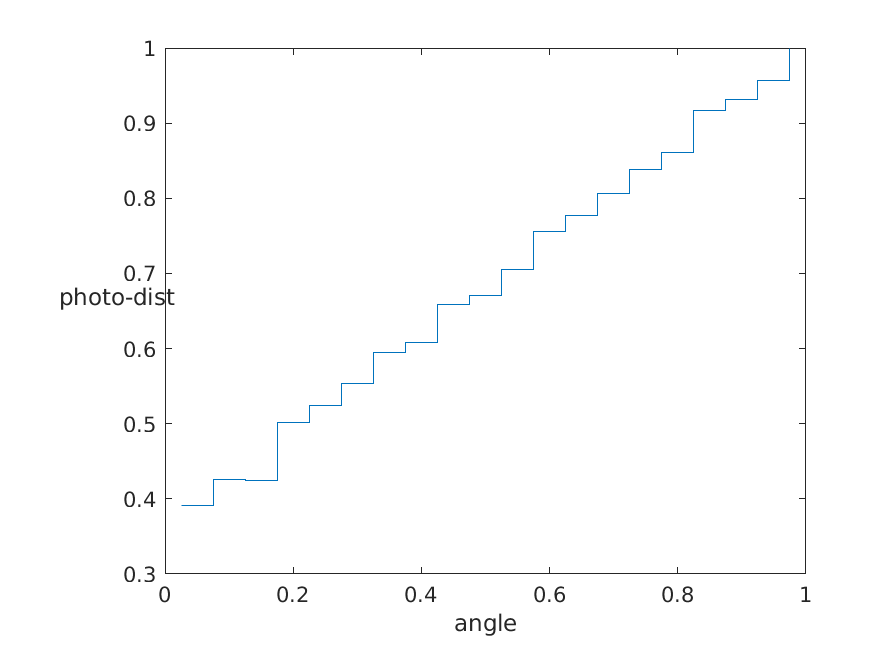
\includegraphics[width=0.7\textwidth]{../../introductory_exercises/limb_darkening/number_channels20number_photons100000max_opt_depth10.png}
\caption{histogram for \texttt{mu}}
\label{2D_mu}
\end{figure}
Figure \ref{2D_mu} is according to what is expected $I = I_0(0.4+0.6\mu)$

\newpage
\subsubsection{3D Code}
What changes is this: 
\begin{itemize}
\item introduction of a new angle $\phi$
\item the optical depth has to be updated according to $\phi$ also
\end{itemize}

\begin{figure}[!htp]
\centering
\begin{minipage}{.5\textwidth}
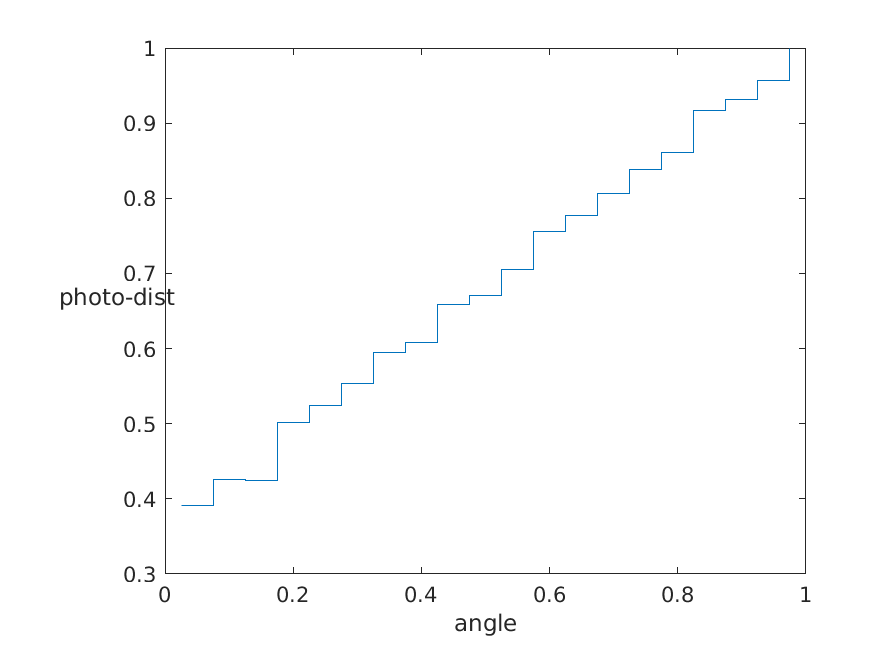
\includegraphics[width=\textwidth]{../../introductory_exercises/limb_darkening/number_channels20number_photons100000max_opt_depth10.png}
\caption{histogram for \texttt{mu}}
\label{3D_mu}
\end{minipage}%
\begin{minipage}{.5\textwidth}
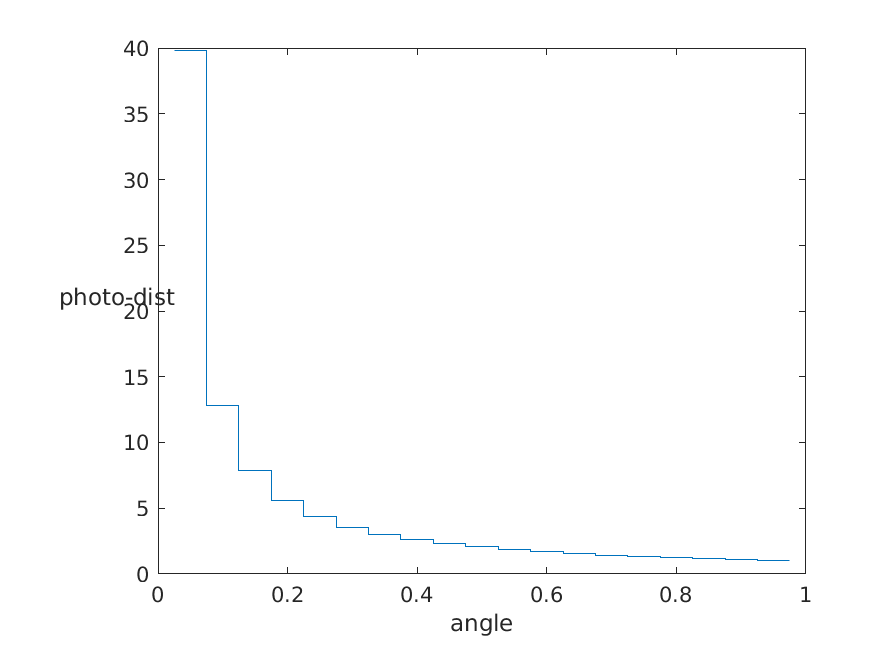
\includegraphics[width=\textwidth]{../../introductory_exercises/limb_darkening/PHI_number_channels20number_photons100000max_opt_depth10.png}
\caption{histogram for \texttt{phi}}
\label{3D_phi}
\end{minipage}
\end{figure}

Figure \ref{3D_mu} and Figure \ref{3D_phi} are according to what is expected, namely $I = I_0(0.4+0.6\mu)$ and a uniform distribution for $phi$, which corresponds to a $I \sim \frac{1}{\phi}$


\newpage
\section{Investigation of program: pcyg.f90}
\subsection{Overview of variables}
\begin{center}
\centering
{\tabulinesep=1.5mm
\begin{tabu}{|c|c|c|}
\hline 
name & explanation \\ \hline \hline

\multicolumn{2}{|c|}{\cellcolor{orange} paramaters} \\ \hline
xk0 & \\ \hline
alpha & velocity profile parameter \\ \hline
beta & velocity profile parameter \\ \hline \hline

\multicolumn{2}{|c|}{\cellcolor{orange} start frequency of the photon} \\ \hline
xstart & start frequency \\ \hline
vmin & \\ \hline
vmax  & \\ \hline

\multicolumn{2}{|c|}{\cellcolor{orange}angle of the photon} \\ \hline
xmuestart & start angle \\ \hline
xmuein & incident angle \\ \hline
xmueou & outward angle \\ \hline
\cellcolor{yellow} pstart & impact parameter \\ \hline
xnew & new photon frequency \\ \hline \hline

\multicolumn{2}{|c|}{\cellcolor{orange} optical depth} \\ \hline
tau & optical depth \\ \hline

\multicolumn{2}{|c|}{\cellcolor{orange} number of photons admin} \\ \hline
nphot & number of photons\\ \hline
nin & photons scattered back into core \\ \hline
nout & photons escaped \\ \hline \hline

\multicolumn{2}{|c|}{\cellcolor{orange} functions} \\ \hline
func & velocity profile \\ 
	& distance from center of star $r$ \\ \hline
	
xmueout & outwards (scattered) angle \\ 
& xk0 \\ 
& alpha \\ 
& r \\ 
& v \\ 
& sigma \\ \hline
\end{tabu}}
\end{center}

\newpage
\subsection{Mathematical things that are noteworthy}

\subsubsection{General working}
\begin{center}
\begin{tikzpicture}
[node distance=2.5cm,auto,>=latex']
    \node [int] (a) {\texttt{pcyg.f90}};
    \node (b) [left of=a,node distance=4cm, coordinate] {a};
    \node (c) [right of=a,node distance=4cm, coordinate] {a};
    \path[->] (b) edge node {\texttt{xstart}} (a);
    \path[->] (a) edge node {\texttt{xnew}} (c);
\end{tikzpicture}
\end{center}
The photons are sorted according to \texttt{xnew}.
In general, the flux is dependent on $\mu$ and the frequency $x$.


\noindent\fbox{
  \parbox{\textwidth}{
  make formula 
}}

\begin{itemize}
\item I think that it satisfies $N(x)dx \sim I(x)xdx$
\item We are thus interested in $F_{\lambda} = F_{\nu}$
\end{itemize}


\subsubsection{Practical formula}
\begin{itemize}
\item emission angle $\mu = \cos(\theta)$
\item according p-ray $p = \sqrt{1-\mu^2} = \sin(\theta)$
\item incident angle $\texttt{xmuein} = \sqrt{1-\left(\frac{pstart}{r}\right)^2}$
\end{itemize}

\subsubsection{Geometry \& Symmetry assumptions}
\begin{itemize}
\item spherical geometry
\end{itemize}


\newpage
\subsection{Exercises}
\subsubsection{Investigation of original code}
In original version of the code, all photons are released isotropially from the photosphere.

\begin{figure}[!htp]
\centering
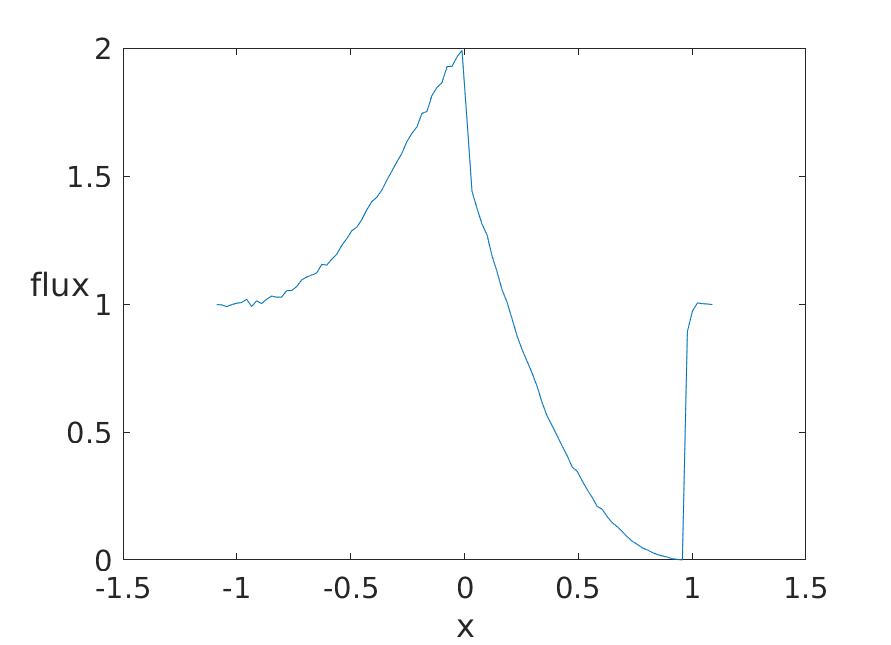
\includegraphics[width=0.5\textwidth]{../../introductory_exercises/P_Cygni_profile_UV_resonance/npot6xk0100alpha0beta1test0.png}
\caption{Original version of the code}
\end{figure}

\newpage
\subsubsection{First adaptation: what if all photons are released radially from photosphere?}
\label{PCYG FIRST adaptation}

\paragraph{\underline{Release photons radially: numerical MC experiments}}
What would happen with line-profile, if you assumed all photons
were released radially from photopshere?
\begin{itemize}
\item In other words $\texttt{xmuestart} = 1$. Results in Figure \ref{PCyg_mu_eq_1}.
\item This is implemented under the test case \texttt{test\_number=1}.
\end{itemize}

\begin{figure}[!htbp]
\centering
\begin{subfigure}{.5\textwidth}
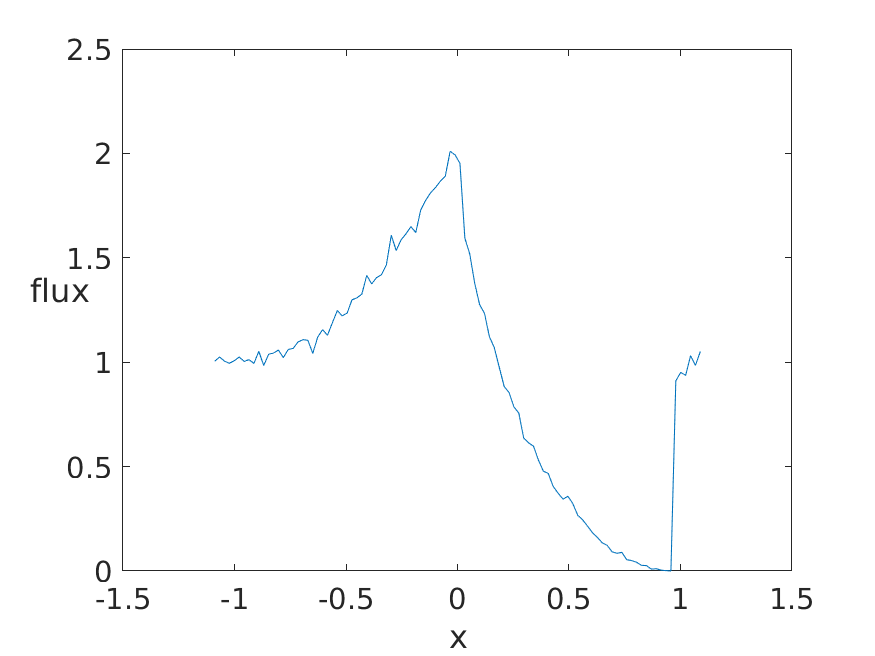
\includegraphics[width=1\textwidth]{../../introductory_exercises/P_Cygni_profile_UV_resonance/npot5xk0100alpha0beta1test1.png}
\caption{First adaptation}
\end{subfigure}%
\begin{subfigure}{.5\textwidth}
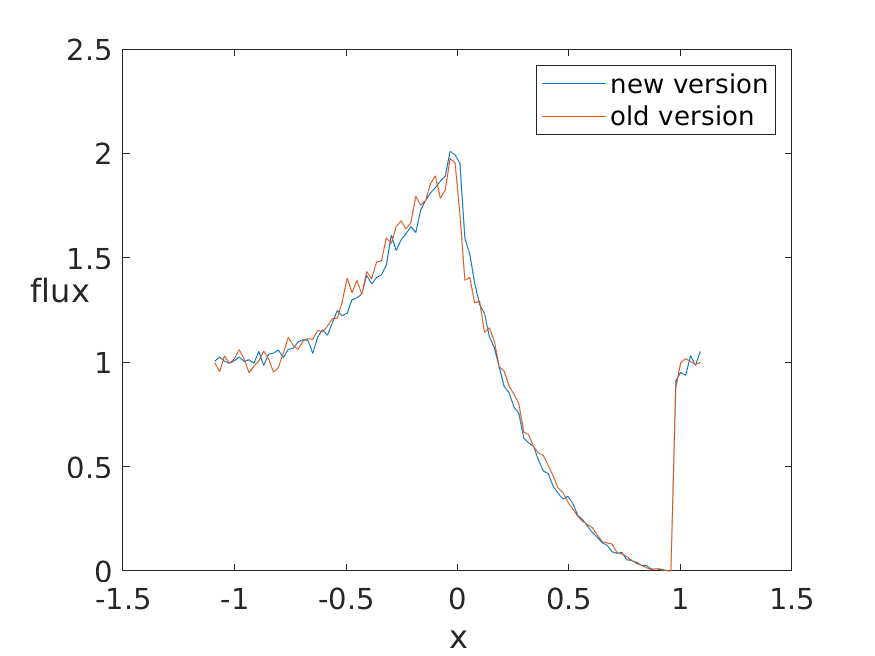
\includegraphics[width=1\textwidth]{../../introductory_exercises/P_Cygni_profile_UV_resonance/npot5xk0100alpha0beta1test10.png}
\caption{Same plot (together with output of initial version)}
\end{subfigure}
\label{PCyg_mu_eq_1}
\caption{The number of photons equals $10^{5}$}
\end{figure}


\paragraph{\underline{Derive analytic expression}} See also slide  26/49 [Sundqvist course material]. 
\begin{itemize}
\item since \texttt{xmuein = 1} we have for the velocity profile 
\begin{equation}
v = v_{\infty}(1-b/r)^{\beta}
\label{velocity_profile}
\end{equation}
A scaled version of the Equation (\ref{velocity_profile}) yields 
\begin{equation}
u = \frac{v(r)}{v_{\infty}} = \left(1 - \frac{r_{\infty}}{r} \right)^{\beta} 
\label{u_profile}
\end{equation}
with $u \in [0..1]$

\item Doppler shift for the frequency of the photons: $x_{CMF} = x_{REF} - \mu u$.
\item Condition for resonance from Sobolov approximation (to be studied later): $\boxed{x_{CMF}= 0}$ thus 
\begin{equation}
x_{REF} = \mu u
\label{analytic_profile}
\end{equation}
or thus $x_{REF} = \boxed{u_{\text{interaction}}}$ and than solve Equation \ref{u_profile} for $r_{\text{interaction}}$

\item If $\mu = 1$ then 
\begin{equation}
x = \left(1 - \frac{r_{\infty}}{r} \right)^{\beta}
\end{equation}
\begin{equation*}
x^{-\beta} = 1 - \frac{r_{\infty}}{r}
\end{equation*}
\begin{equation*}
r(1-x^{-\beta}) = r_{\infty}
\end{equation*}
\begin{equation}
\boxed{r(x) = \frac{r_{\infty}}{1-x^{-\beta}}}
\end{equation} 

\item From the location of interaction $r$, the incident angle can be calculated
\begin{equation}
\texttt{xmuein} = \sqrt{1-\left[\frac{\texttt{pstart}}{r}\right]^2} = \sqrt{1 - \left[ \frac{\sqrt{1-\texttt{xmuestart}^2}}{r} \right]^2}
\end{equation}
Now also taking into account that \texttt{xmuestart = 1} then yields
\begin{equation}
\texttt{xmuein = 1}
\end{equation}

\item The calculation of the optical depth goes as follows:
\begin{equation}
\tau = \frac{\texttt{xkO}}{rv^{2-\alpha}(1+\texttt{xmuein}^2 \sigma)}
\end{equation}
Now also taking into account that \texttt{xmuestart = 1} gives
\begin{equation}
\tau = \frac{\texttt{xk0}}{rv^2(1+\sigma)}
\end{equation}

where $\boxed{v(x) = \left(1 - \frac{b}{r} \right)^{\beta}}$ 
\quad and $\frac{dv}{dr} = \frac{\beta b}{r^2}\left( 1 - \frac{b}{r} \right)^{\beta - 1}$  \\
and $\sigma(x) = \frac{dv}{dr}\frac{r}{v}-1$ 
thus $\boxed{\sigma(x) = \frac{\beta b}{r}\left( 1-\frac{b}{r}\right)^{-1}}$

\item Conclusion: $\tau(x)$ is only dependent on $x$ and not on \texttt{xmuestart} or \texttt{xmuein}.

\item \texttt{xmueou} follows the distribution as given by the function \texttt{xmueout}, namely
\begin{equation}
p(x) = \frac{1-e^{-\tau}}{\tau}
\end{equation}
with $\tau = \frac{\texttt{tau0}}{1+\texttt{X}^2 \sigma}$ where $\texttt{X}$ is a random number, so actually this comes down to
\begin{equation}
\boxed{p(x) = \frac{1-e^{-\frac{\tau_0}{1+x^2\sigma(x)}}}{\frac{\tau_0}{1+x^ 2\sigma(x)}}}
\end{equation}

\item Finally one can combine these results to get the distribution of the photons according to the frequency $x$ via the relation 
\begin{equation}
\texttt{xnew = xstart + v(xmueou-xmuein) = xstart + v(xmueou -1)}
\end{equation}
\end{itemize}

\underline{Via this link, you can go back to the exercises overview: Section \ref{Overview_Part_2}.}


\newpage
\subsubsection{Second adaptation: isotropic scattering}
\label{isotropic_scattering}
What would happen to line-profile, is you assumed scattering
was isotropic 
\\(i.e., NOT following Sobolev-distrobution)
\begin{itemize}
\item test case number 2
\end{itemize}

\begin{figure}[!htbp]
\centering
\begin{subfigure}{.5\textwidth}
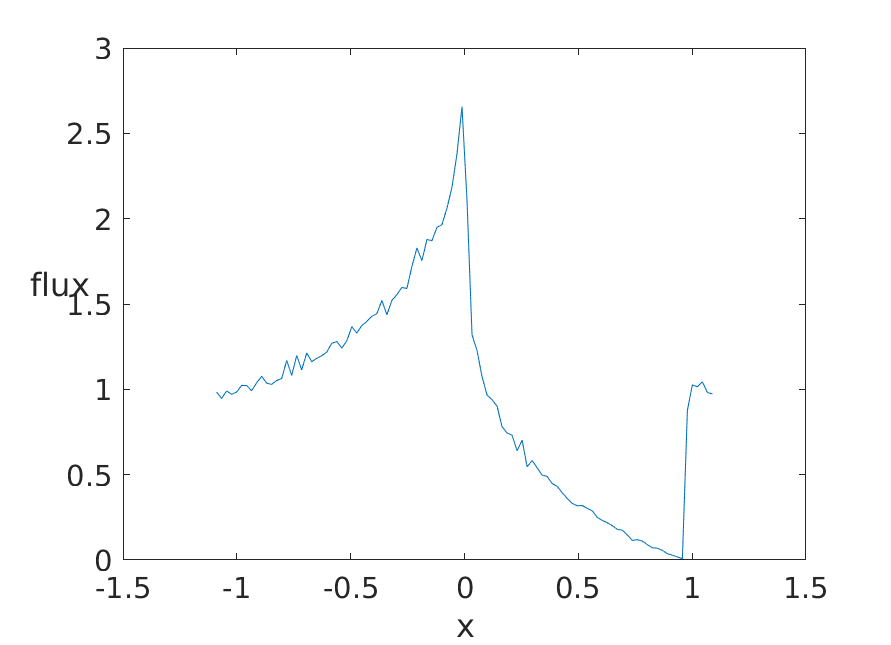
\includegraphics[width=1\textwidth]{../../introductory_exercises/P_Cygni_profile_UV_resonance/npot5xk0100alpha0beta1test2.png}
\caption{Second adaptation}
\end{subfigure}%
\begin{subfigure}{.5\textwidth}
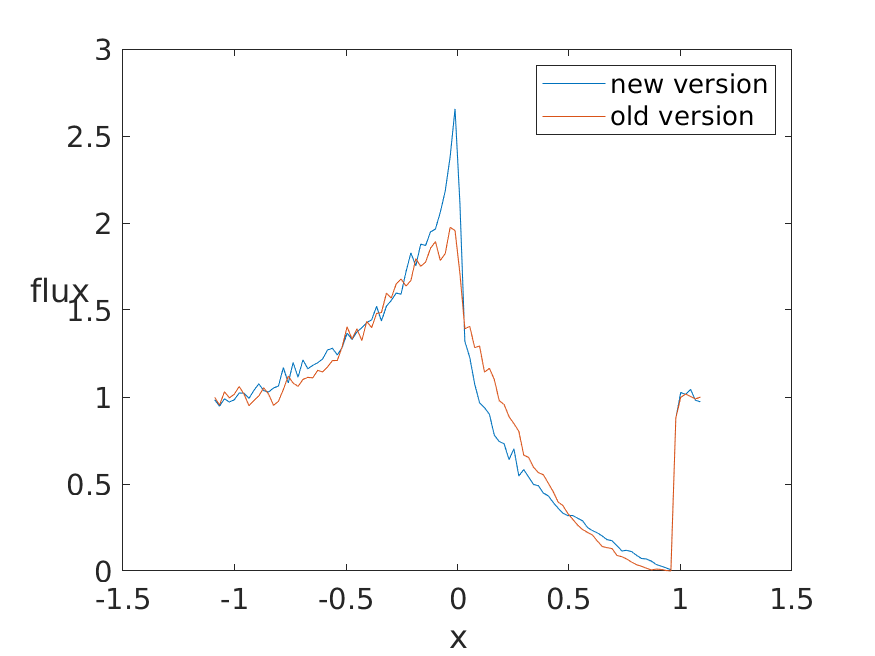
\includegraphics[width=1\textwidth]{../../introductory_exercises/P_Cygni_profile_UV_resonance/npot5xk0100alpha0beta1test20.png}
\caption{Same plot (together with output of initial version)}
\end{subfigure}
\label{PCyg_mu_eq_1}
\caption{The number of photons equals $10^{5}$}
\end{figure}

The \textit{grosso modo} form has not changed, although the scaling has changed.

\newpage
\subsubsection{Third adaptation: introduction of Eddington limb-darkening}
\label{Eddington limb darkening adaptation}
Put Eddington limb-darkening in. What happens? 

\paragraph{General (introductory) discussion: Eddington limb darkening}
The data are taken from Christensen, 2015.
\begin{itemize}
\item the source function $S= <I> = a + b\tau_{\nu}$ with $a= \frac{\sigma}{2 \pi}T_{eff}^4$ and $b = \frac{3 \sigma}{4 \pi}T_{eff}^4$
\item solve the equation
\item this yields $\frac{I(\theta)}{I(0)} = \frac{a+b\cos(\theta)}{a+b} = \frac{2}{5} + \frac{3}{5}\cos(\theta)$
\end{itemize}

\begin{figure}[!htp]
\centering
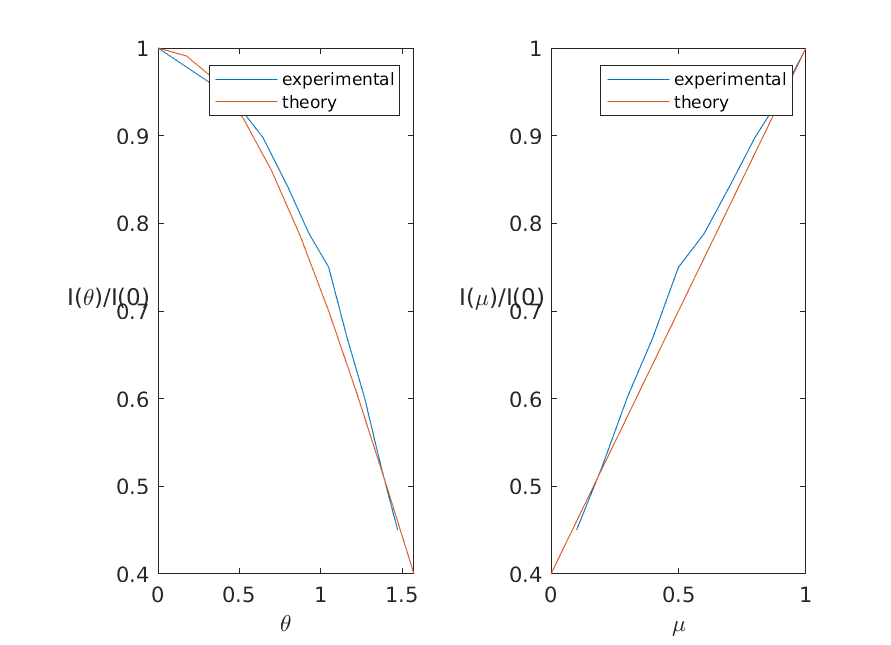
\includegraphics[width=0.7\textwidth]{../../introductory_exercises/P_Cygni_profile_UV_resonance/Eddington_limb_darkening.png}
\caption{Eddington limb darkening (two times the same plot with $\mu =  \cos(\theta)$ }
\end{figure}

\paragraph{Construction of probability distribution corresponding to Eddington limb darkening}

\begin{enumerate}
\item Let us thus first review the emmission case where \underline{the flux in each direction is isotropic} i.e. $I(\theta) = I$ (as experimented in paragraph \ref{isotropic_scattering})
\begin{itemize}
\item the specific intensity is defined as $I_{\nu}(\mu) = \frac{dE_{\nu}}{\cos(\theta) dA dt d\nu d\Omega} = \frac{dE_{\nu}}{\mu dA dt d\nu d\Omega}$ 
\item the flux $F_{\nu} = \int_{\Omega} I_{\nu} \cos(\theta) d\Omega$ is in this case isotropic thus
\begin{equation}
\xi = \int_0^{\mu} F_{\nu} d\mu = \int_0^{\mu} \int_{\Omega} I_{\nu} \cos(\theta) d\Omega d\mu = A \int_0^{\mu} \mu d\mu   
\end{equation}
together with the condition that $\mu$ satisfies a probability distribution: 
\begin{equation}
1 = \int_{-1}^{1} F_{\nu} d\mu = \int_{-1}^{1} \int_{\Omega} I_{\nu} \cos(\theta) d\Omega d\mu = \frac{A}{2}
\label{isotropic_flux_isotropic_intensity_prob_dist}
\end{equation}
thus $A=2$. Photons need to be sampled according to $\mu d\mu$.
\end{itemize}

\item Now we look at a new case where the photons need to be emitted following a distrubution that corresponds to $I(\theta) = I(0)(0.4+0.6\cos(\theta))$. 
\begin{itemize}
\item in this case the flux $F_{\nu} = \int_{\Omega} I_{\nu} \cos(\theta) d\Omega$ is isotropic but also satisfies
\begin{equation}
F_{\nu} = \int_{\Omega} I_{\nu}(0)[0.4+0.6\cos(\theta)] \cos(\theta) d\Omega
\end{equation} 
\noindent\fbox{
  \parbox{0.8\textwidth}{
I am not sure about the correctness of the assumption of isotropy of the flux}}
\begin{equation}
\xi = \int_0^{\mu} F_{\nu} d\mu = A \int_0^{\mu} (0.4+0.6\mu) \mu d\mu   
\end{equation}
subject to the normalisation condition -very similar to Equation (\ref{isotropic_flux_isotropic_intensity_prob_dist}) - that
\begin{equation}
1 = \int_{-1}^{1} F_{\nu} d\mu = \frac{2A}{5} + \frac{A}{3} = \frac{11A}{15}
\end{equation}
thus $A = \frac{15}{11}$. Photons need to be sampled according to
\begin{equation}
(0.4+0.6\mu)\mu d\mu
\label{prob_dist_Eddington}
\end{equation}
\end{itemize}

In the code \texttt{pcyg.f90} this corresponds to \texttt{test\_number = 3} (not yet implemented). 

The results of an accept-reject method that samples the probability distribution in Equation (\ref{prob_dist_Eddington}).

\begin{figure}[!htp]
\centering
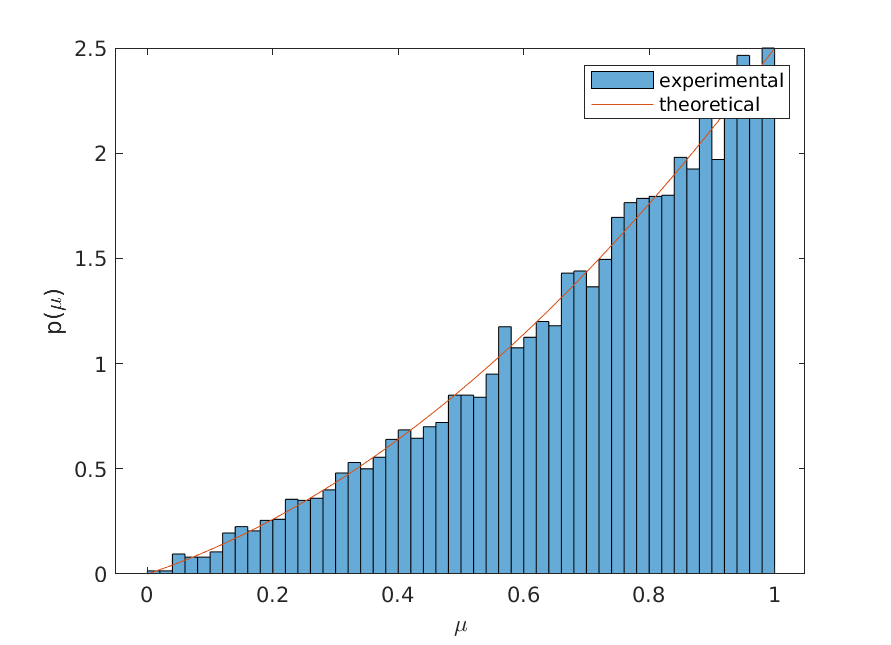
\includegraphics[width=0.7\textwidth]{../../introductory_exercises/P_Cygni_profile_UV_resonance/Eddington_accept_reject.png}
\caption{Accept-reject method for Eddington limb darkening}
\end{figure}

\end{enumerate}



\underline{Via this link, you can go back to the exercises overview: Section \ref{Overview_Part_2}.}

\newpage
\subsubsection{Fourth adaptaion: photospheric line-profile}
Challening: Put photospheric line-profile (simple Gaussian) in
!What happens? Test on xk0=0 (opacity =0) case.

\begin{itemize}
\item test case number 4 (not yet implemented)
\end{itemize}

\newpage
\subsubsection{Convergence analysis}
\label{convergence_analysis}

\begin{figure}[!htp]
\centering
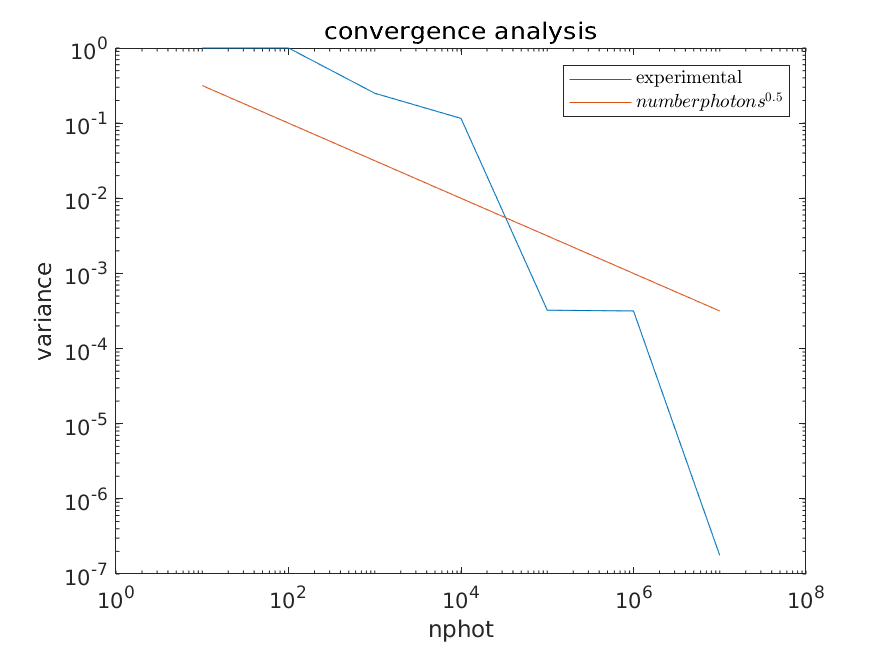
\includegraphics[width=0.65\textwidth]{../../introductory_exercises/P_Cygni_profile_UV_resonance/test0_convergence.png}
\caption{Original version of the code: convergence analysis (xk0=0)}
\end{figure}

\underline{Via this link, you can go back to the exercises overview: Section \ref{Overview_Part_2}.}

\newpage
\section{Milic Exercises}
\subsection{Lecture 7}
\begin{enumerate}
\item Derive expressions for the emergent radiation when properties are the following:
\begin{itemize}
\item optically thin slab at all wavelengths
\item wavelength-independent incident radiation
\end{itemize}
Solution: see slide 14?

\item Derive ralations between Einstein coefficients.

\item Calculate electron density in atmosphere from FALC model
\end{enumerate}


\newpage
\section{Mass loss from inhomogeneous hot star winds (Sundqvist)}
\begin{itemize}
\item GOAL: synthesis of UV resonance lines from inhomogeneous 2D winds
\begin{itemize}
\item clumped in density
\item clumped in velocity
\item effects of non-void inter-clump medium
\end{itemize}

\item WIND MODELS
\begin{itemize}
\item symmetry assumptions
\begin{itemize}
\item 1D: spherical symmetry
\item 2D: symmetry in $\Phi$
\end{itemize}

\item models
\begin{enumerate}

\item time-dependent radiation-hydrodynamic from Puls and Owocki (POF)
\begin{itemize}
\item 1D
\item isothermal flow
\item perturbations triggered by photospheric sound waves
\end{itemize}

\item time-dependent radiation-hydrodynamic from Feldmeier (FPP)
\begin{itemize}
\item 1D
\item treatment of energy equation
\item perturbations triggered by photospeheric sound waves or Langevin perturbagions (photospheric turbulence)
\end{itemize}

\item stochastic model, clumped in density
\begin{itemize}
\item smooth winds with $v_{\beta} = (1-b/r)^{\beta}$ with $\beta = 1$
\item clumping factor $f_{cl}$
\end{itemize}

\item stochastic model, clumped in density and in velocity (non-monotonic velocity field)
\begin{itemize}
\item smooth winds with $v_{\beta} = (1-b/r)^{\beta}$ with $\beta = 1$
\item clumping factor $f_{cl}$
\end{itemize}
\end{enumerate}

\end{itemize}

\item RADIATIVE TRANSFER (MC-2D)
\end{itemize}

\newpage
\section{Asymptotic preserving Monte Carlo methods for radiative transfer equation in diffusion limit (Dimarco+ 2018)}
\subsection{Goldstein-Taylor}
\subsection{Radiative transfer}

\end{document}